\subsection*{\textbf{Задание для самостоятельной работы}}

\begin{enumerate}
    \item Решите дифференциальное уравнение $y'' - 7y' + 12 = -e^{4x}$
    \begin{figure}[H]
        \renewcommand{\figurename}{Рисунок}
        \centering{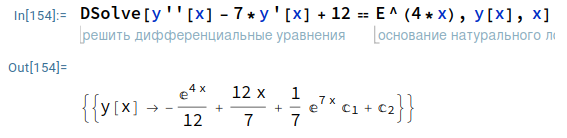
\includegraphics[scale=0.70]{body/img/self_2_1.png}}
        \label{fig:image_self_2_1}
    \end{figure}
    \item Постройте графики функции, являющихся частными решениями предыдущего дифференциального уравнения, объявив
    $C[1] = C[2] = 1,2$ и $3$ (то есть три графика).
    \begin{figure}[H]
        \renewcommand{\figurename}{Рисунок}
        \centering{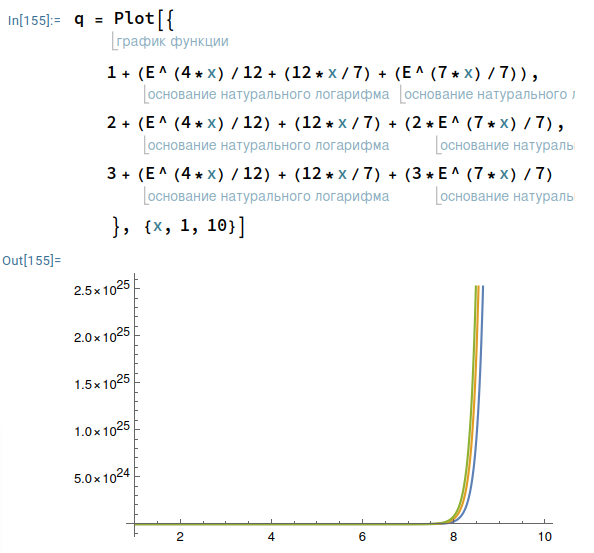
\includegraphics[scale=0.50]{body/img/self_2_2.png}}
        \label{fig:image_self_2_2}
    \end{figure}
    \item Построение график функции эвольвенты (развертки окружности); параметр $a$ (радиус развёртываемой окружности)
    задайте самостоятельно:
    \[
        \begin{cases}
            X(t) = a\cdot(\cos t + t\cdot\sin t) \\
            Y(t) = a\cdot(\sin t - t\cdot\cos t) \\
        \end{cases}
    \]
    \begin{figure}[H]
        \renewcommand{\figurename}{Рисунок}
        \centering{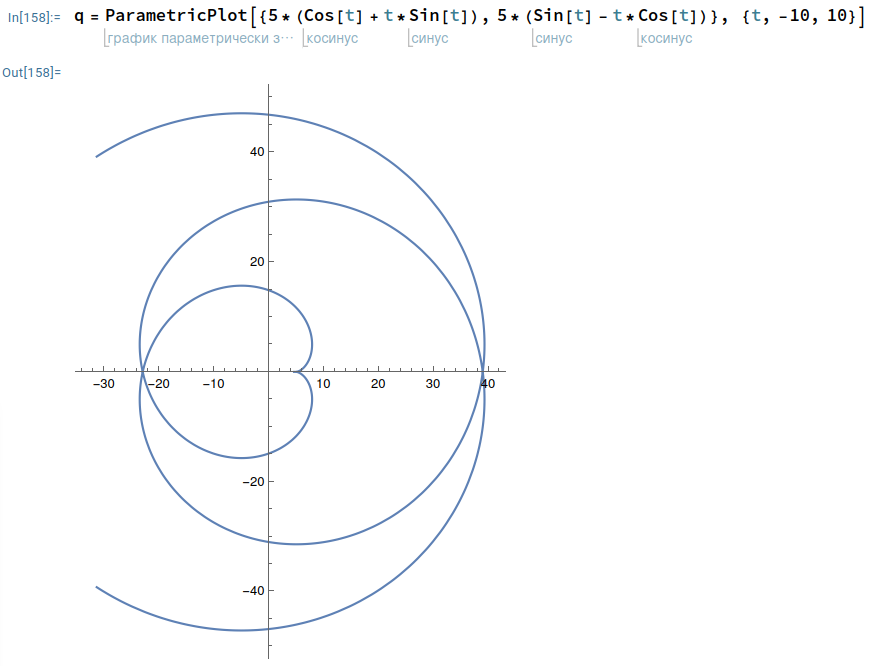
\includegraphics[scale=0.50]{body/img/self_2_3.png}}
        \label{fig:image_self_2_3}
    \end{figure}
    \item Постройте поверхность \[f(x,y) = \frac{1}{x+y};\]
    пределы изменения аргументов поберите самостоятельно.
    \begin{figure}[H]
        \renewcommand{\figurename}{Рисунок}
        \centering{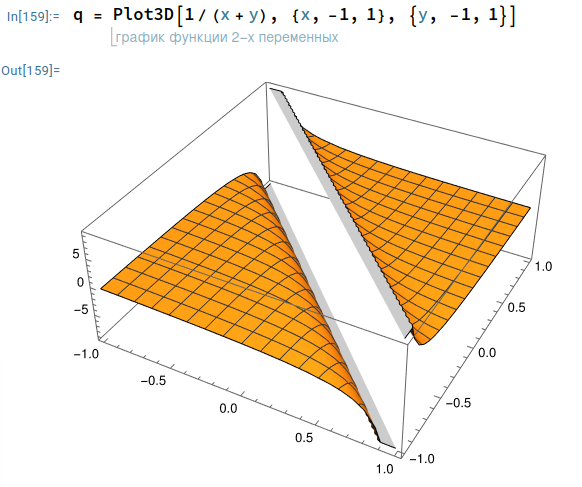
\includegraphics[scale=0.50]{body/img/self_2_4.png}}
        \label{fig:image_self_2_4}
    \end{figure}
\end{enumerate}